\documentclass[12pt,a4paper]{article}
\usepackage{cmap}
\usepackage[T2A]{fontenc}
\usepackage[utf8]{inputenc}
\usepackage[russian]{babel}
\usepackage{amsmath,amssymb,geometry,graphicx,float,hyperref,array,longtable}
\usepackage[labelfont=bf]{caption}
\captionsetup{skip=5pt}
\geometry{left=2cm,right=2cm,top=2cm,bottom=2cm}
\hypersetup{hidelinks,pdftitle={Лабораторная работа 1 Статическая оптимизация Вариант 11},
pdfauthor={Иванов Никита Михайлович}}
\addto\captionsrussian{\renewcommand{\figurename}{Рисунок}}
\captionsetup[table]{justification=raggedright,singlelinecheck=false}
\makeatletter
\def\tagform@#1{\maketag@@@{\ignorespaces#1\unskip\@@italiccorr}}
\makeatother
\setlength{\emergencystretch}{2em}
\setlength{\intextsep}{8pt}
\graphicspath{{results/}}
\newcommand{\norm}[1]{\left\lVert#1\right\rVert_2}
\title{Лабораторная работа №1\\Поиск минимума с помощью методов статической оптимизации\\Вариант 11}
\author{Иванов Никита Михайлович\\Группа R3436}
\date{16 октября 2026 г.}
\begin{document}
\maketitle
\newpage
\tableofcontents
\newpage

\section{Постановка задачи}
В работе рассматривается статическая задача оптимизации критерия
\begin{equation}
J(x,u)=8x^2+6u^2+4xu+x+3u-10
\end{equation}
с функцией ограничения
\begin{equation}
c(x,u)=3x-u^2+1.
\end{equation}
Необходимо найти глобальный минимум без ограничений, с ограничением
$c(x,u)=0$ и с ограничением $c(x,u)\leq0$. Затем требуется выполнить
пошаговый расчёт минимума $J_1(x,u)=J(x,u)$ без ограничений методом
Ньютона--Рафсона и методом наискорейшего спуска при двух различных
постоянных шагах, обеспечивающих апериодическую и колебательную сходимость.

\section{Поиск минимума без ограничений}
\subsection{Необходимое условие}
Градиент критерия имеет вид
\[
\nabla J(x,u)=
\begin{pmatrix}16x+4u+1\\4x+12u+3\end{pmatrix}.
\]
Из условия стационарности $\nabla J=0$ получаем систему
\[
\begin{cases}
16x+4u+1=0,\\
4x+12u+3=0.
\end{cases}
\]
Её решение: $x^*=0$, $u^*=-1/4$.

\subsection{Достаточное условие и результат}
Матрица Гессе постоянна:
\[
H=\begin{pmatrix}16&4\\4&12\end{pmatrix},\qquad
\Delta_1=16>0,\qquad \Delta_2=\det H=176>0.
\]
По критерию Сильвестра $H$ положительно определена. Следовательно,
$J$ строго выпукла на всей плоскости, а стационарная точка является
единственным глобальным минимумом:
\begin{equation}
x^*=0,\qquad u^*=-\frac14=-0.25,\qquad
J^*=-\frac{83}{8}=-10.375.
\end{equation}
\newpage

\section{Минимум при ограничении в виде равенства}
\subsection{Условия Лагранжа}
Для ограничения $3x-u^2+1=0$ составим функцию Лагранжа:
\[
L(x,u,\lambda)=J(x,u)+\lambda(3x-u^2+1).
\]
Множитель равенства $\lambda$ заранее не ограничивается по знаку.
Необходимые условия имеют вид
\begin{equation}
\begin{cases}
16x+4u+1+3\lambda=0,\\
4x+12u+3-2\lambda u=0,\\
3x-u^2+1=0.
\end{cases}
\end{equation}
Из третьего и первого уравнений выразим
\[
x=\frac{u^2-1}{3},\qquad
\lambda=-\frac{16u^2+12u-13}{9}.
\]
Подстановка во второе уравнение даёт
\begin{equation}
32u^3+36u^2+82u+15=0.
\end{equation}

\subsection{Проверка глобальности минимума}
Подставим ограничение непосредственно в критерий:
\[
\varphi(u)=J\!\left(\frac{u^2-1}{3},u\right)
=\frac{8u^4+12u^3+41u^2+15u-85}{9}.
\]
Тогда
\[
\varphi'(u)=\frac{32u^3+36u^2+82u+15}{9},
\]
\[
\varphi''(u)=\frac{96u^2+72u+82}{9}
=\frac{32}{3}\left(u+\frac38\right)^2+\frac{137}{18}>0.
\]
Функция $\varphi$ строго выпукла и стремится к $+\infty$ при $|u|\to\infty$.
Поэтому уравнение $\varphi'(u)=0$ имеет ровно один действительный корень;
он задаёт единственный глобальный минимум на всей параболе $c=0$.

\subsection{Результат}
\begin{align*}
u^*&=-0.196978642820,& x^*&=-0.320399804758,\\
\lambda^*&=1.638103815800,& J^*&=-9.604836264941.
\end{align*}
\newpage

\section{Минимум при ограничении в виде неравенства}
\subsection{Условия Куна--Таккера}
Допустимая область задаётся неравенством
\[
3x-u^2+1\leq0,\qquad x\leq\frac{u^2-1}{3}.
\]
Для лагранжиана $L=J+\lambda c$ условия Куна--Таккера имеют вид
\begin{equation}
\begin{cases}
16x+4u+1+3\lambda=0,\\
4x+12u+3-2\lambda u=0,\\
c(x,u)\leq0,\quad \lambda\geq0,\quad \lambda c(x,u)=0.
\end{cases}
\end{equation}
\textbf{Неактивное ограничение.}
При $\lambda=0$ получаем безусловный минимум $(0,-1/4)$, но
\[
c(0,-1/4)=\frac{15}{16}=0.9375>0.
\]
Следовательно, эта точка недопустима.

\textbf{Активное ограничение.}
При $c=0$ получаем решение предыдущего раздела. Для него
$\lambda^*=1.638103815800>0$, поэтому все условия Куна--Таккера выполнены.
Градиент ограничения $(3,-2u)^{\mathsf T}$ нигде не обращается в нуль.

\subsection{Достаточность для глобального минимума}
Область $c\leq0$ невыпукла, поэтому одной проверки условий
Куна--Таккера недостаточно. При найденном $\lambda^*$ гессиан
лагранжиана постоянен:
\[
H_L=\begin{pmatrix}16&4\\4&12-2\lambda^*\end{pmatrix}
=\begin{pmatrix}16&4\\4&8.723792368\end{pmatrix}.
\]
Его главные угловые миноры положительны:
\[
\Delta_1=16>0,\qquad
\det H_L=176-32\lambda^*=123.580677894>0.
\]
Следовательно, $L(z,\lambda^*)$ строго выпукла на всей плоскости,
а найденная стационарная точка $z^*=(x^*,u^*)^{\mathsf T}$ является
её единственным глобальным минимумом. Для любой допустимой точки $z$
\[
J(z)=L(z,\lambda^*)-\lambda^*c(z)
\geq L(z,\lambda^*)\geq L(z^*,\lambda^*)=J(z^*).
\]
Это доказывает единственность глобального минимума задачи с неравенством:
\[
x^*=-0.320399804758,\quad u^*=-0.196978642820,\quad
J^*=-9.604836264941.
\]
\newpage

\section{Пошаговый расчёт методом Ньютона--Рафсона}
Для всех численных методов выбраны одна начальная точка
$z_0=(0,0)^{\mathsf T}$ и общий критерий остановки
\[
\norm{\nabla J(z_k)}\leq10^{-6}.
\]
Формула метода Ньютона--Рафсона:
\[
z_{k+1}=z_k-H^{-1}\nabla J(z_k),\qquad
H^{-1}=\frac1{176}\begin{pmatrix}12&-4\\-4&16\end{pmatrix}.
\]
При $z_0=(0,0)^{\mathsf T}$ имеем
\[
\nabla J(z_0)=\begin{pmatrix}1\\3\end{pmatrix},\qquad
H^{-1}\nabla J(z_0)=\begin{pmatrix}0\\1/4\end{pmatrix},\qquad
z_1=\begin{pmatrix}0\\-1/4\end{pmatrix}.
\]
\begin{table}[H]\centering
\caption{Пошаговый расчёт методом Ньютона--Рафсона}
\small\setlength{\tabcolsep}{4pt}
\begin{tabular}{r|r|r|r|r}\hline
$k$&$x_k$&$u_k$&$J_k$&$\norm{\nabla J(z_k)}$\\\hline
% BEGIN NEWTON
0 & $0.000000000$ & $0.000000000$ & $-10.000000000000$ & $3.162278\cdot10^{0}$ \\
1 & $0.000000000$ & $-0.250000000$ & $-10.375000000000$ & $0$ \\
% END NEWTON
\hline\end{tabular}
\end{table}
В точке $z_1$ градиент равен нулю. Метод достигает точного минимума
за одну итерацию, поскольку гессиан квадратичного критерия постоянен.

\section{Градиентный поиск минимума}
\subsection{Выбор шага}
Используем метод наискорейшего спуска с постоянным параметром $\gamma$:
\[
\begin{cases}
x_{k+1}=x_k-\gamma(16x_k+4u_k+1),\\
u_{k+1}=u_k-\gamma(4x_k+12u_k+3).
\end{cases}
\]
Для ошибки $e_k=z_k-z^*$ получаем $e_{k+1}=(I-\gamma H)e_k$.
Собственные значения $H$ равны
\[
\mu_1=14-2\sqrt5=9.527864045,\qquad
\mu_2=14+2\sqrt5=18.472135955.
\]
Условие сходимости:
\[
0<\gamma<\frac2{\mu_2}=0.108271182.
\]
При $\gamma=0.05<1/\mu_2=0.054135591$ оба множителя $1-\gamma\mu_i$
положительны. При $\gamma=0.09$ один множитель отрицателен, а модули
обоих меньше единицы. Эти шаги дают требуемые режимы сходимости.
\newpage

\subsection{Апериодическая сходимость при шаге 0.05}
Первый шаг:
\[
z_1=z_0-0.05\nabla J(z_0)
=(-0.05,-0.15)^{\mathsf T},\qquad J_1=-10.315.
\]
Множители изменения собственных составляющих ошибки равны
\[
r_1=0.523606798,\qquad r_2=0.076393202.
\]
Оба числа находятся между нулём и единицей.
Полный расчёт до выполнения критерия остановки приведён в таблице.

\begin{center}\small\setlength{\tabcolsep}{4pt}
\begin{longtable}{r|r|r|r|r}
\caption{Апериодическая сходимость при $\gamma=0.05$}\\
\hline $k$&$x_k$&$u_k$&$J_k$&$\norm{\nabla J(z_k)}$\\\hline
\endfirsthead
\hline $k$&$x_k$&$u_k$&$J_k$&$\norm{\nabla J(z_k)}$\\\hline
\endhead
% BEGIN AP
0 & $0.000000000$ & $0.000000000$ & $-10.000000000000$ & $3.162278\cdot10^{0}$ \\
1 & $-0.050000000$ & $-0.150000000$ & $-10.315000000000$ & $1.077033\cdot10^{0}$ \\
2 & $-0.030000000$ & $-0.200000000$ & $-10.358800000000$ & $5.556978\cdot10^{-1}$ \\
3 & $-0.016000000$ & $-0.224000000$ & $-10.370560000000$ & $2.908745\cdot10^{-1}$ \\
4 & $-0.008400000$ & $-0.236400000$ & $-10.373782720000$ & $1.523029\cdot10^{-1}$ \\
5 & $-0.004400000$ & $-0.242880000$ & $-10.374666265600$ & $7.974680\cdot10^{-2}$ \\
6 & $-0.002304000$ & $-0.246272000$ & $-10.374908502016$ & $4.175597\cdot10^{-2}$ \\
7 & $-0.001206400$ & $-0.248048000$ & $-10.374974914540$ & $2.186371\cdot10^{-2}$ \\
8 & $-0.000631680$ & $-0.248977920$ & $-10.374993122468$ & $1.144799\cdot10^{-2}$ \\
9 & $-0.000330752$ & $-0.249464832$ & $-10.374998114428$ & $5.994243\cdot10^{-3}$ \\
10 & $-0.000173184$ & $-0.249719782$ & $-10.374999483044$ & $3.138627\cdot10^{-3}$ \\
11 & $-0.000090680$ & $-0.249853276$ & $-10.374999858269$ & $1.643406\cdot10^{-3}$ \\
12 & $-0.000047481$ & $-0.249923174$ & $-10.374999961142$ & $8.604986\cdot10^{-4}$ \\
13 & $-0.000024861$ & $-0.249959774$ & $-10.374999989347$ & $4.505629\cdot10^{-4}$ \\
14 & $-0.000013018$ & $-0.249978937$ & $-10.374999997079$ & $2.359178\cdot10^{-4}$ \\
15 & $-0.000006816$ & $-0.249988971$ & $-10.374999999199$ & $1.235282\cdot10^{-4}$ \\
16 & $-0.000003569$ & $-0.249994225$ & $-10.374999999780$ & $6.468019\cdot10^{-5}$ \\
17 & $-0.000001869$ & $-0.249996976$ & $-10.374999999940$ & $3.386699\cdot10^{-5}$ \\
18 & $-0.000000978$ & $-0.249998417$ & $-10.374999999983$ & $1.773299\cdot10^{-5}$ \\
19 & $-0.000000512$ & $-0.249999171$ & $-10.374999999996$ & $9.285112\cdot10^{-6}$ \\
20 & $-0.000000268$ & $-0.249999566$ & $-10.374999999999$ & $4.861748\cdot10^{-6}$ \\
21 & $-0.000000140$ & $-0.249999773$ & $-10.375000000000$ & $2.545644\cdot10^{-6}$ \\
22 & $-0.000000074$ & $-0.249999881$ & $-10.375000000000$ & $1.332917\cdot10^{-6}$ \\
23 & $-0.000000039$ & $-0.249999938$ & $-10.375000000000$ & $6.979242\cdot10^{-7}$ \\
% END AP
\hline\end{longtable}
\end{center}
Критерий остановки впервые выполнен при $k=23$:
\[
\norm{\nabla J(z_{23})}=6.979242\cdot10^{-7}.
\]
Апериодичность означает отсутствие смены знака у собственных составляющих ошибки.
Для отдельной координаты это не требует монотонности на каждом шаге.
\newpage

\subsection{Колебательная сходимость при шаге 0.09}
Первый шаг: $z_1=(-0.09,-0.27)^{\mathsf T}$, $J_1=-10.3006$.
Множители равны $0.142492236$ и $-0.662492236$. Отрицательный множитель
вызывает затухающие колебания относительно минимума.

\begin{center}\footnotesize\setlength{\tabcolsep}{4pt}
\begin{longtable}{r|r|r|r|r}
\caption{Колебательная сходимость при $\gamma=0.09$}\\
\hline $k$&$x_k$&$u_k$&$J_k$&$\norm{\nabla J(z_k)}$\\\hline
\endfirsthead
\hline $k$&$x_k$&$u_k$&$J_k$&$\norm{\nabla J(z_k)}$\\\hline
\endhead
% BEGIN OSC
0 & $0.000000000$ & $0.000000000$ & $-10.000000000000$ & $3.162278\cdot10^{0}$ \\
1 & $-0.090000000$ & $-0.270000000$ & $-10.300600000000$ & $1.634136\cdot10^{0}$ \\
2 & $0.046800000$ & $-0.216000000$ & $-10.344177280000$ & $1.066365\cdot10^{0}$ \\
3 & $-0.032832000$ & $-0.269568000$ & $-10.361509212160$ & $7.059568\cdot10^{-1}$ \\
4 & $0.021490560$ & $-0.236615040$ & $-10.369079702578$ & $4.676756\cdot10^{-1}$ \\
5 & $-0.014274432$ & $-0.258807398$ & $-10.372401620691$ & $3.098310\cdot10^{-1}$ \\
6 & $0.009451414$ & $-0.244156613$ & $-10.373859582123$ & $2.052606\cdot10^{-1}$ \\
7 & $-0.006262241$ & $-0.253869980$ & $-10.374499475204$ & $1.359835\cdot10^{-1}$ \\
8 & $0.004148579$ & $-0.247435995$ & $-10.374780321688$ & $9.008804\cdot10^{-2}$ \\
9 & $-0.002748417$ & $-0.251698609$ & $-10.374903584076$ & $5.968263\cdot10^{-2}$ \\
10 & $0.001820803$ & $-0.248874681$ & $-10.374957683440$ & $3.953928\cdot10^{-2}$ \\
11 & $-0.001206268$ & $-0.250745514$ & $-10.374981427433$ & $2.619446\cdot10^{-2}$ \\
12 & $0.000799143$ & $-0.249506102$ & $-10.374991848575$ & $1.735363\cdot10^{-2}$ \\
13 & $-0.000529426$ & $-0.250327203$ & $-10.374996422373$ & $1.149664\cdot10^{-2}$ \\
14 & $0.000350741$ & $-0.249783230$ & $-10.374998429794$ & $7.616438\cdot10^{-3}$ \\
15 & $-0.000232363$ & $-0.250143608$ & $-10.374999310843$ & $5.045831\cdot10^{-3}$ \\
16 & $0.000153939$ & $-0.249904861$ & $-10.374999697532$ & $3.342824\cdot10^{-3}$ \\
17 & $-0.000101983$ & $-0.250063029$ & $-10.374999867248$ & $2.214595\cdot10^{-3}$ \\
18 & $0.000067563$ & $-0.249958244$ & $-10.374999941736$ & $1.467152\cdot10^{-3}$ \\
19 & $-0.000044760$ & $-0.250027663$ & $-10.374999974428$ & $9.719767\cdot10^{-4}$ \\
20 & $0.000029653$ & $-0.249981673$ & $-10.374999988777$ & $6.439270\cdot10^{-4}$ \\
21 & $-0.000019645$ & $-0.250012141$ & $-10.374999995074$ & $4.265967\cdot10^{-4}$ \\
22 & $0.000013015$ & $-0.249991957$ & $-10.374999997838$ & $2.826170\cdot10^{-4}$ \\
23 & $-0.000008622$ & $-0.250005329$ & $-10.374999999051$ & $1.872316\cdot10^{-4}$ \\
24 & $0.000005712$ & $-0.249996470$ & $-10.374999999583$ & $1.240395\cdot10^{-4}$ \\
25 & $-0.000003784$ & $-0.250002339$ & $-10.374999999817$ & $8.217517\cdot10^{-5}$ \\
26 & $0.000002507$ & $-0.249998451$ & $-10.374999999920$ & $5.444041\cdot10^{-5}$ \\
27 & $-0.000001661$ & $-0.250001026$ & $-10.374999999965$ & $3.606635\cdot10^{-5}$ \\
28 & $0.000001100$ & $-0.249999320$ & $-10.374999999984$ & $2.389368\cdot10^{-5}$ \\
29 & $-0.000000729$ & $-0.250000451$ & $-10.374999999993$ & $1.582938\cdot10^{-5}$ \\
30 & $0.000000483$ & $-0.249999702$ & $-10.374999999997$ & $1.048684\cdot10^{-5}$ \\
31 & $-0.000000320$ & $-0.250000198$ & $-10.374999999999$ & $6.947449\cdot10^{-6}$ \\
32 & $0.000000212$ & $-0.249999869$ & $-10.374999999999$ & $4.602631\cdot10^{-6}$ \\
33 & $-0.000000140$ & $-0.250000087$ & $-10.375000000000$ & $3.049207\cdot10^{-6}$ \\
34 & $0.000000093$ & $-0.249999943$ & $-10.375000000000$ & $2.020076\cdot10^{-6}$ \\
35 & $-0.000000062$ & $-0.250000038$ & $-10.375000000000$ & $1.338285\cdot10^{-6}$ \\
36 & $0.000000041$ & $-0.249999975$ & $-10.375000000000$ & $8.866033\cdot10^{-7}$ \\
% END OSC
\hline\end{longtable}
\end{center}
Критерий остановки впервые выполнен при $k=36$:
\[
\norm{\nabla J(z_{36})}=8.866033\cdot10^{-7}.
\]
Хотя координаты колеблются, значение $J$ убывает.
\newpage

\section{Геометрия задачи и траектории поиска}
\begin{figure}[H]\centering
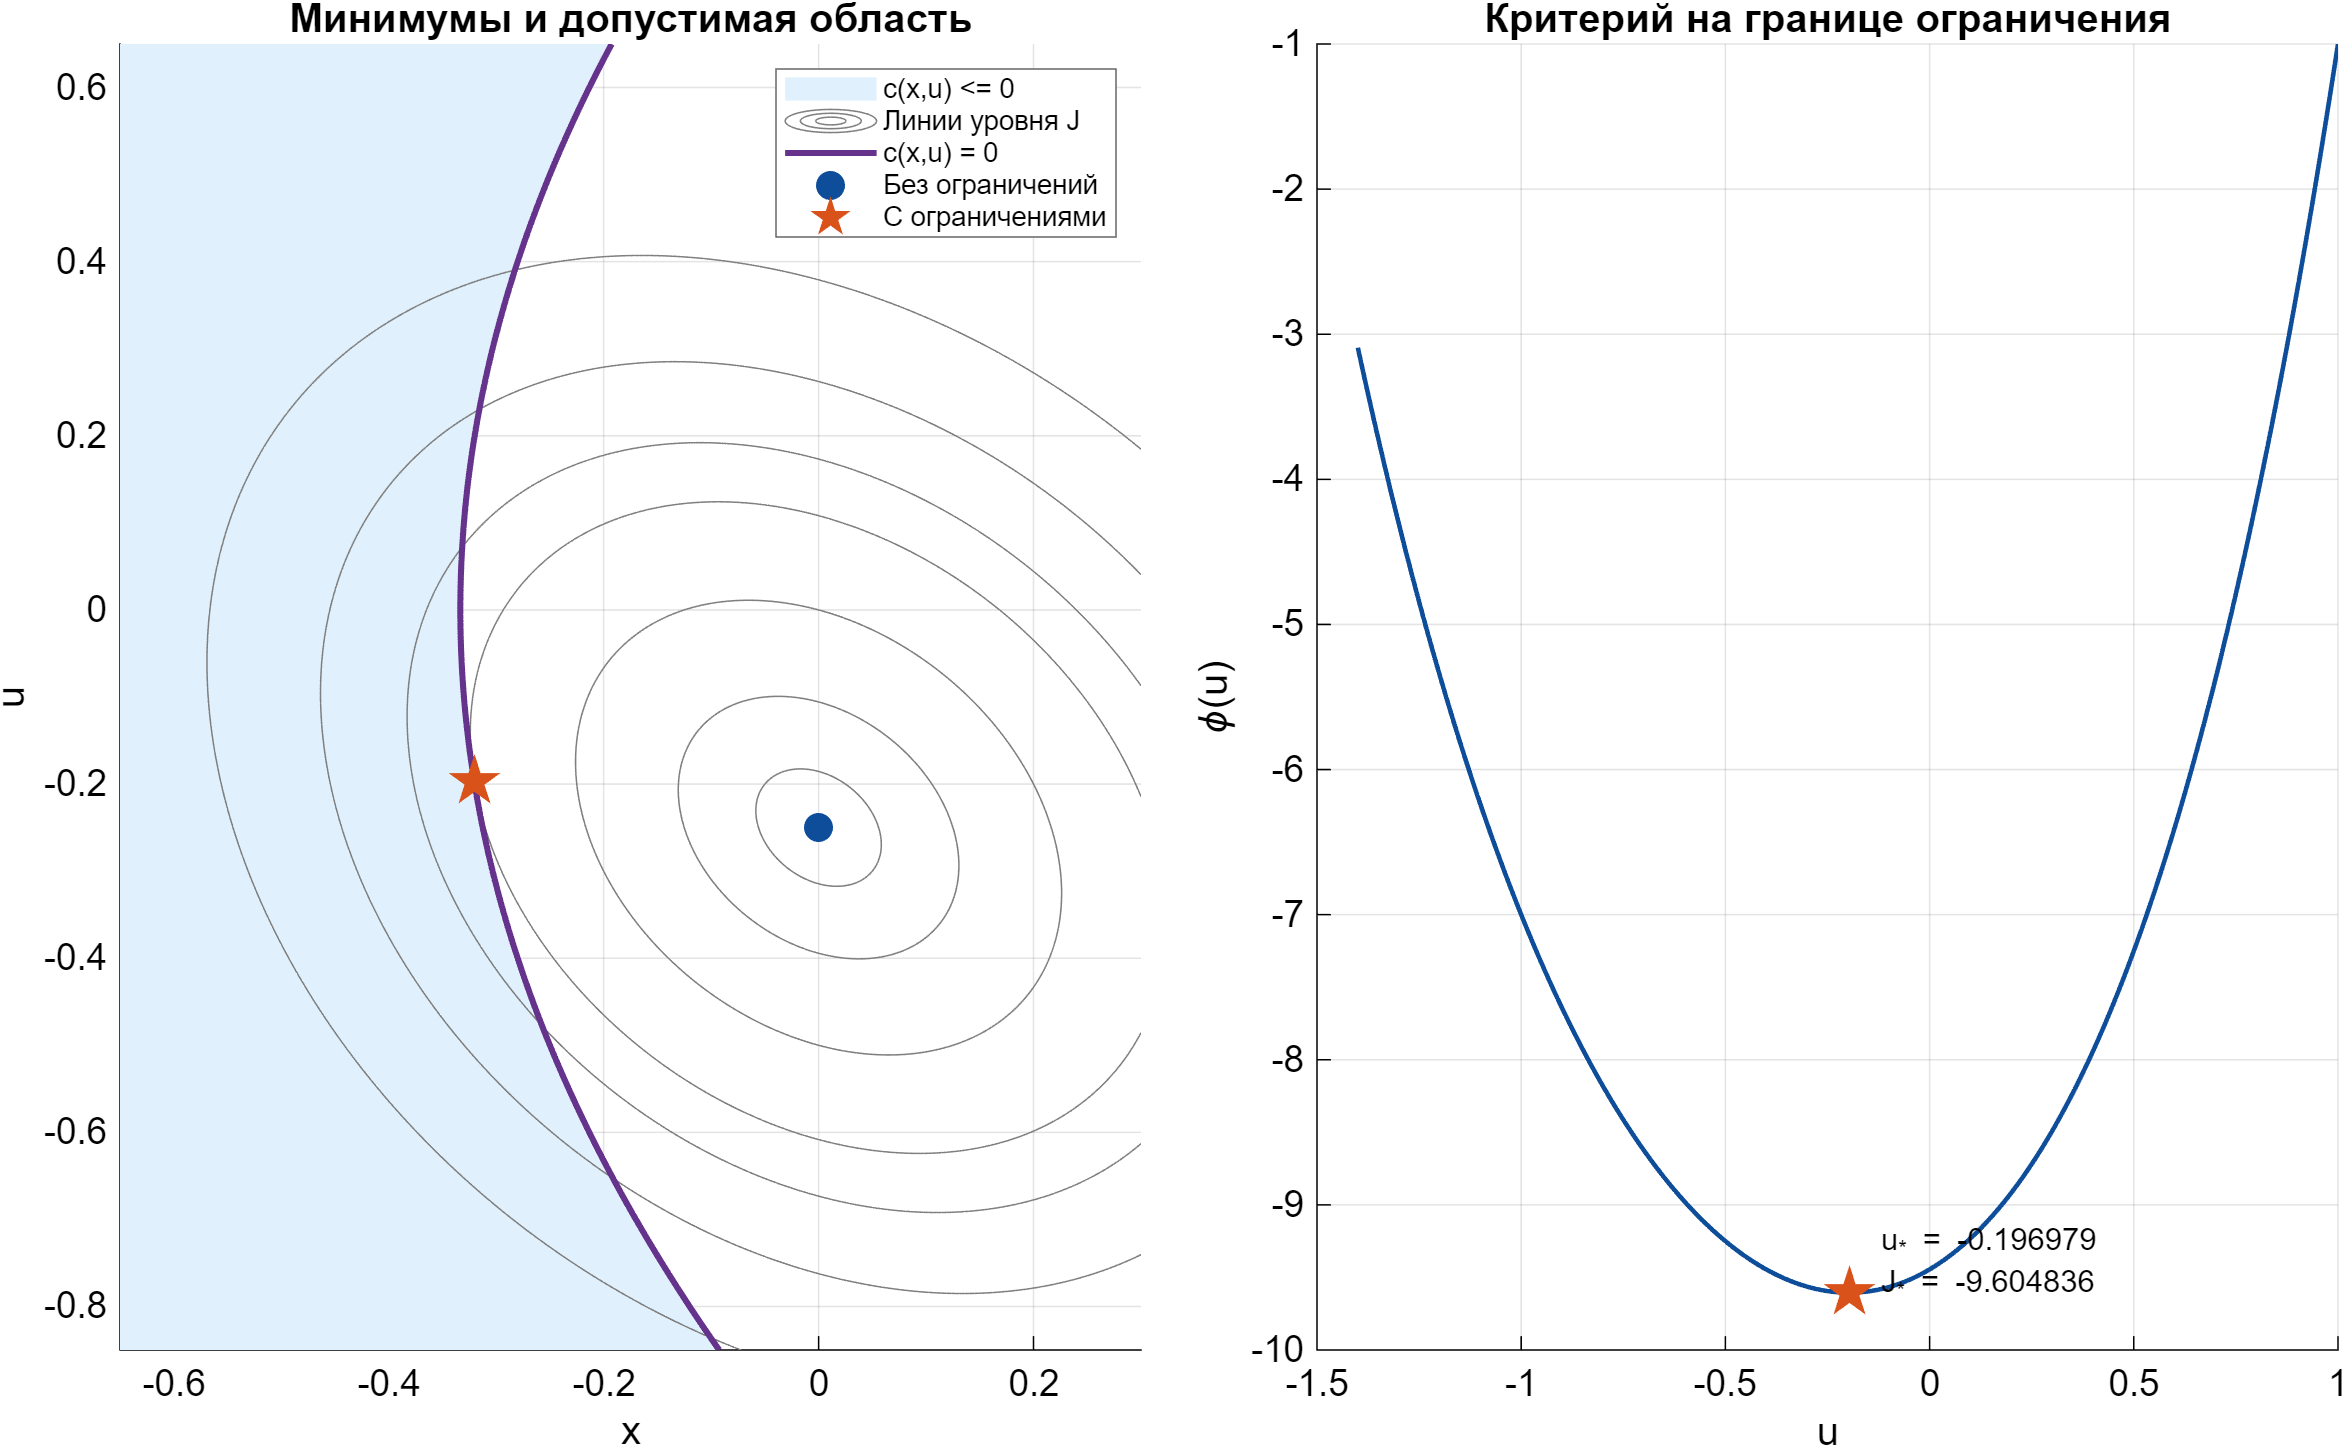
\includegraphics[width=.97\linewidth]{constraints.png}
\caption{Линии уровня критерия, допустимая область $c\leq0$,
безусловный и ограниченный минимумы; справа --- критерий $\varphi$
на границе $c=0$}
\end{figure}
\begin{figure}[H]\centering
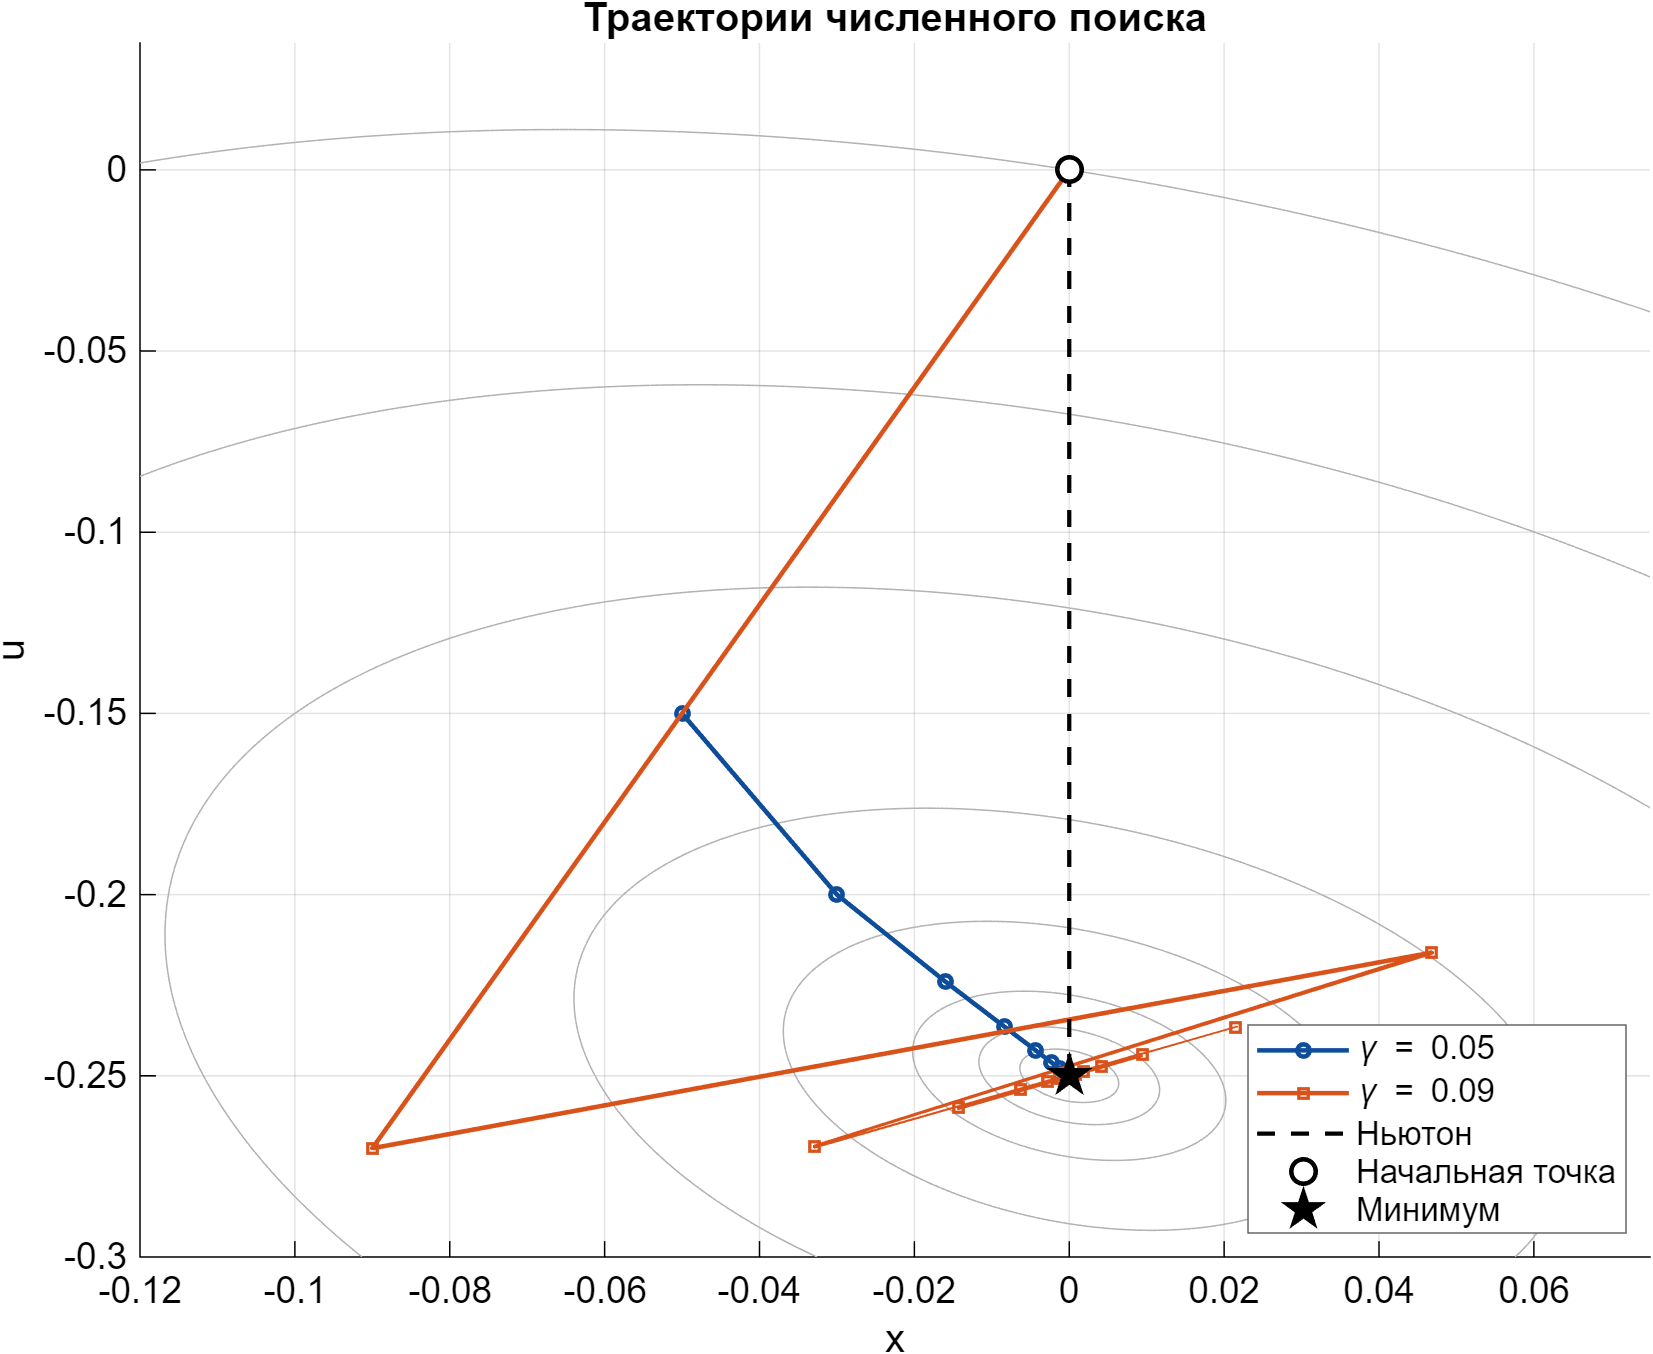
\includegraphics[width=.70\linewidth]{trajectories.png}
\caption{Траектории градиентного поиска при двух шагах
и единственный шаг метода Ньютона из точки $(0,0)$}
\end{figure}
\newpage

\section{Сравнение сходимости}
\begin{figure}[H]\centering
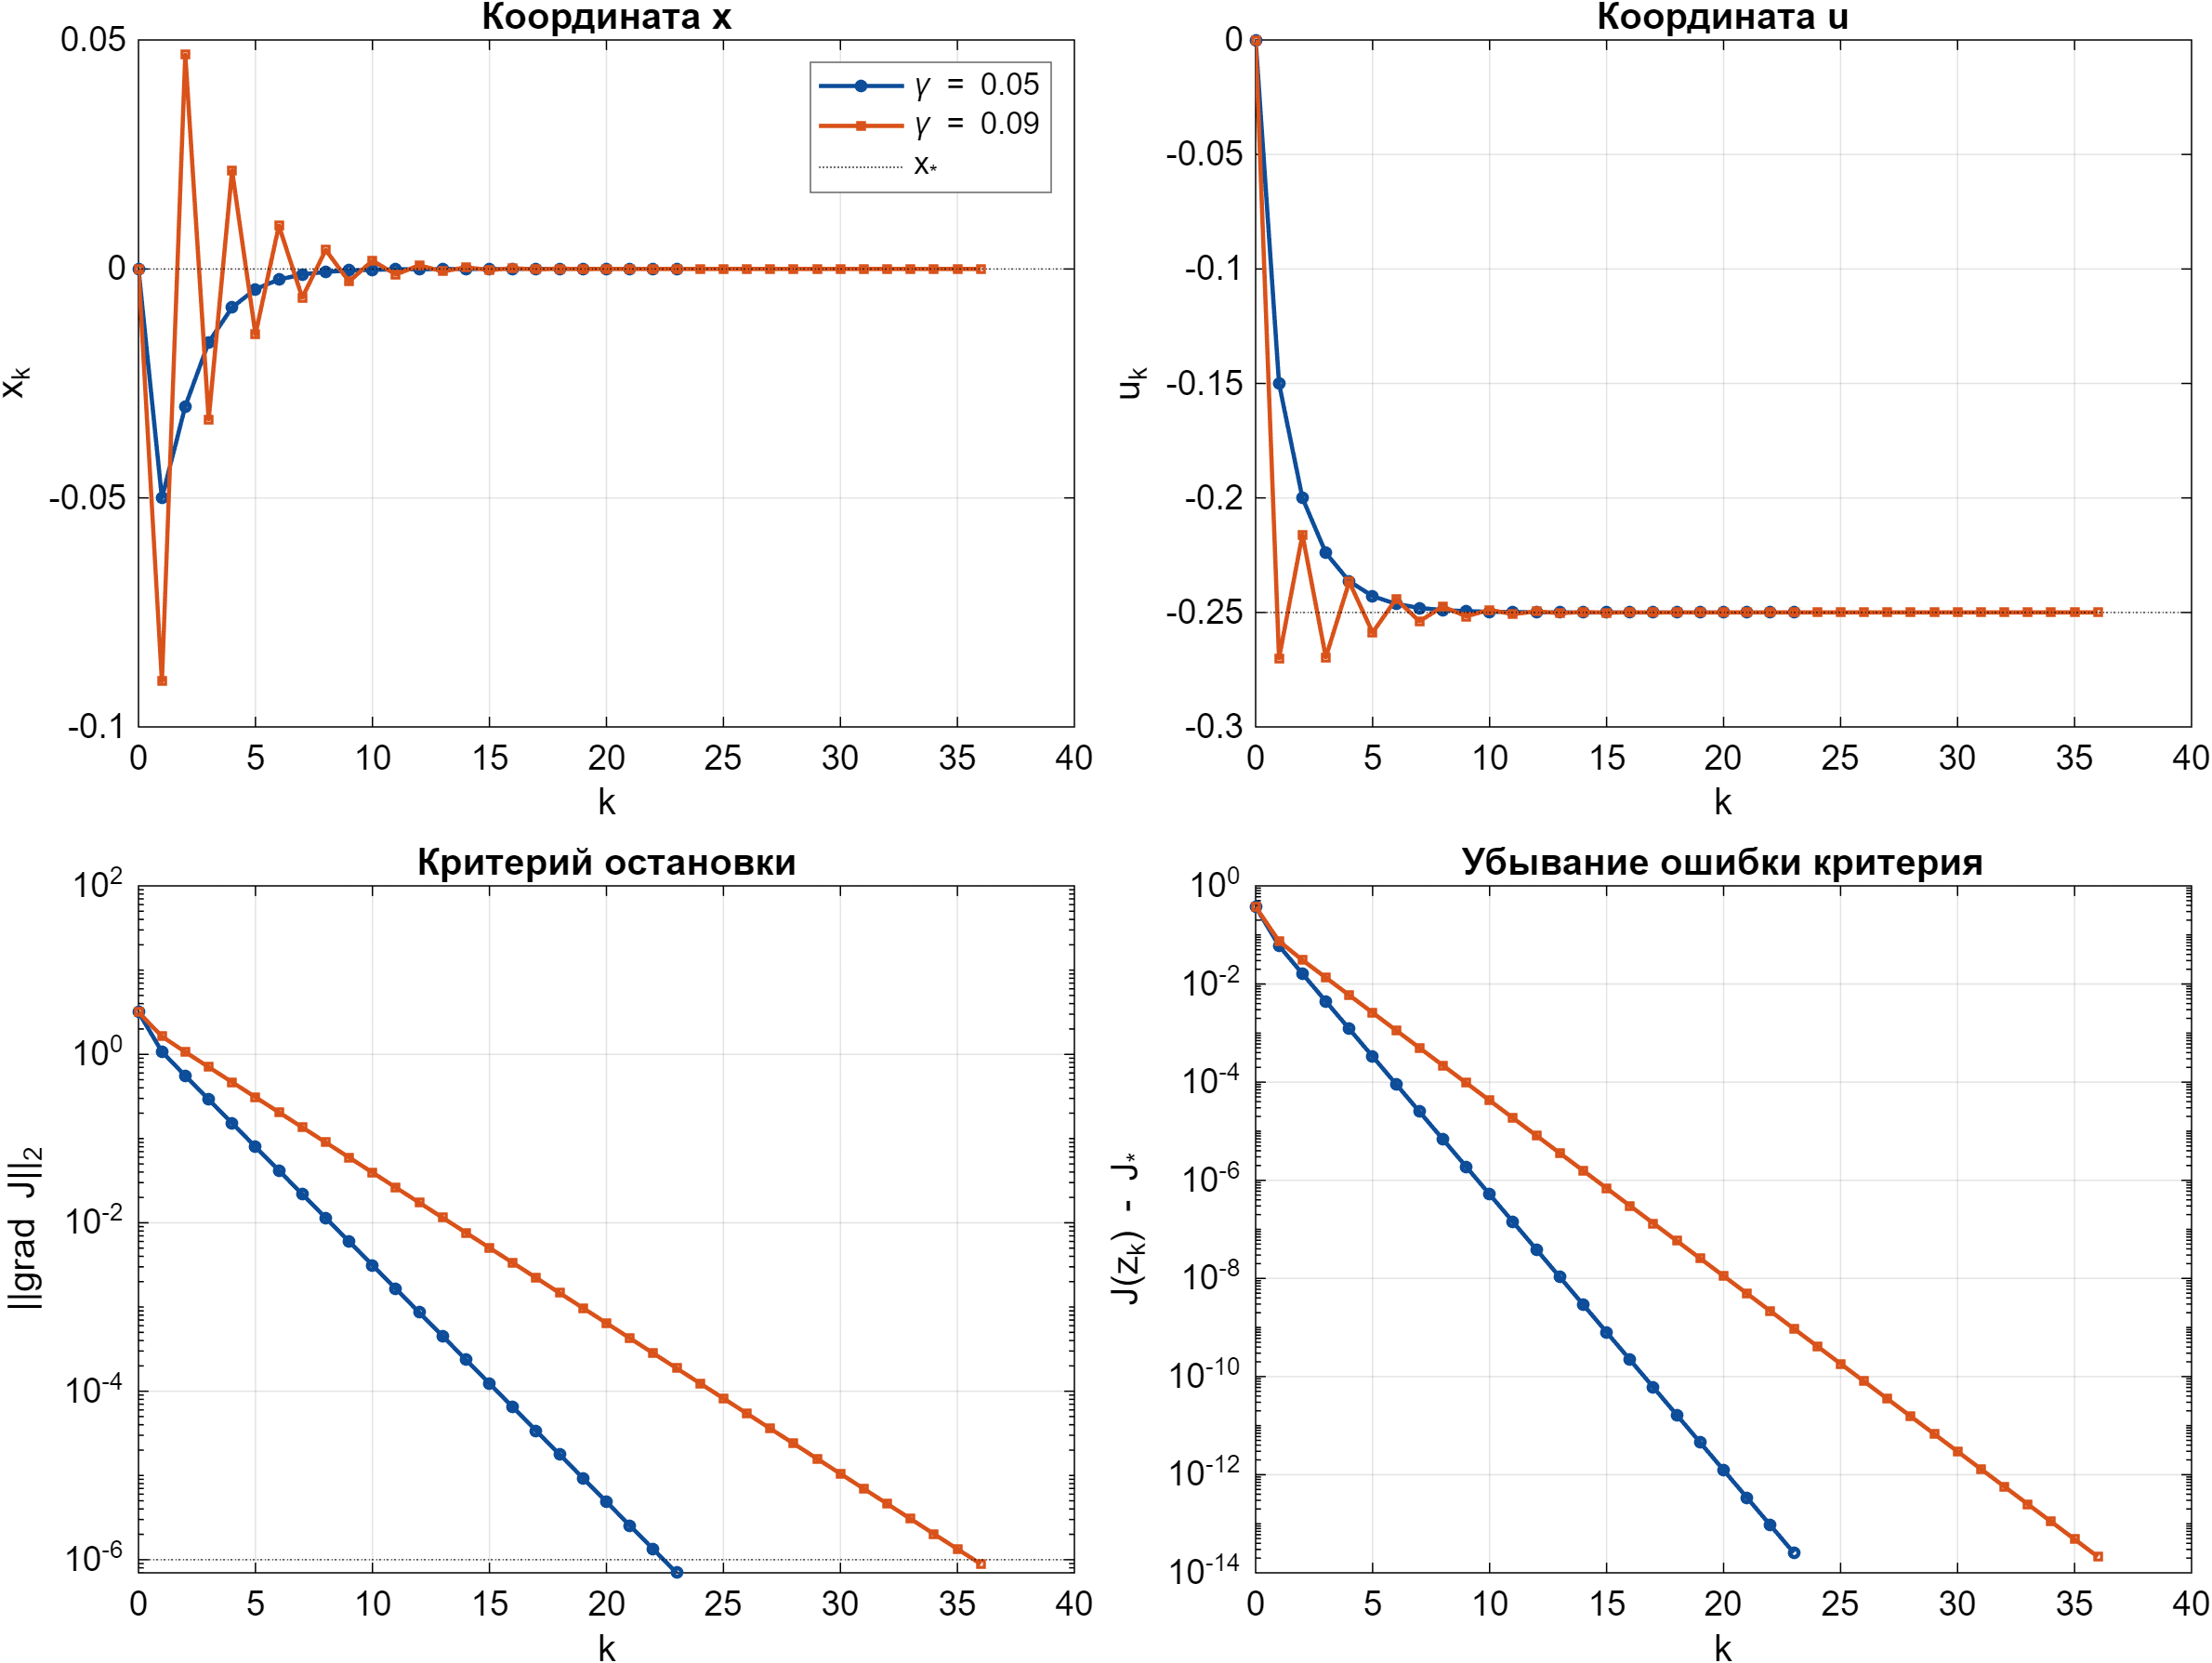
\includegraphics[width=.90\linewidth]{descent.png}
\caption{Изменение координат, нормы градиента и ошибки критерия $J(z_k)-J^*$}
\end{figure}
\begin{table}[H]\centering
\caption{Сравнение численных методов}
\begin{tabular}{l|c|r}\hline
Метод&Число итераций&Итоговый $J$\\\hline
Ньютона--Рафсона&1&$-10.375000000000$\\
Градиентный, $\gamma=0.05$&23&$-10.375000000000$\\
Градиентный, $\gamma=0.09$&36&$-10.375000000000$\\\hline
\end{tabular}
\end{table}
\section{Выводы}
Безусловный минимум равен $-10.375$ в точке $(0,-0.25)$.
Оба ограничения дают минимум $-9.604836265$ в точке
$(-0.320399805,-0.196978643)$. Глобальность доказана:
для равенства --- строгой выпуклостью $\varphi$, для неравенства ---
нижней оценкой через строго выпуклый лагранжиан при $\lambda^*>0$.
Ограничение увеличивает минимум критерия на $0.770163735$.

Метод Ньютона решил квадратичную задачу за один шаг.
Для выбранных постоянных шагов апериодический режим оказался быстрее
колебательного: его спектральный радиус $0.523606798$ меньше
$0.662492236$. Больший шаг сам по себе не обеспечивает более быстрой
сходимости.

\end{document}
